\chapter{Stochastic Interventional Vaccine Efficacy}\label{three}

\section{Introduction}

The core ideas of Chapter~\ref{two} can form a novel approach to studying immune
correlates of protection --- those immunologic markers \textit{causally}
antagonistic to the process of infection~\citep{plotkin2012nomenclature}. In
vaccine efficacy trials of infectious diseases, such analyses can aid in
developing a more nuanced understanding of the differing roles that immunologic
markers can play in impacting vaccine efficacy and, beyond this, elucidate the
mechanism by which the activities of these markers may afford protection. This
analytic framework quantifies vaccine efficacy as the effect attributable to
shifting (upwards or downwards) the immune response distribution (i.e.,
immunologic marker activity) in vaccinees~\citep{hejazi2020efficient}, revealing
the complex interplay between vaccination, immunologic marker activity, and
infection.

To formalize, let us denote by the random variable $O = (W, A, S, Y)$ the data
collected on a single individual in a randomized vaccine efficacy trial,
where $W$ are clinically relevant baseline risk factors for infection (e.g.,
age, body mass index), $A$ is the randomized assignment to placebo or vaccine,
$S$ is the immune response activity of an antibody of interest, and $Y$ is an
indicator of infection. Throughout, we assume that $S$ is the scalar-valued
activity of a particular antibody, as quantified by an established immunoassay,
and is a candidate immune correlate of protection. In measuring $S$, we further
assume that biological material (e.g., drawn blood) for evaluating the activity
of the immunologic marker is taken at an \textit{a priori}-specificed time
post-vaccination. Since such trials often measure the time-to-infection, the
outcome process is generally a composite time-to-event quantity
$\{\tilde{T} = \min(T_F, T_C), \Delta = \mathbb{I}(T_F < T_C)\}$, where $T_F$
and $T_C$ are the (mutually unobservable) failure and censoring times,
respectively, and $\Delta$ is simply the indicator of observed failure. We
simplify this to $Y \coloneqq \mathbb{I}(\Delta = 1)$ (i.e., observed infection)
by the end of the trial.

Leveraging the framework developed in Chapter~\ref{two}, we formulate and
evaluate vaccine efficacy parameters in the context of efficacy trials of the
vaccines produced to counteract the COVID-19 pandemic. The central goal of this
and related statistical analyses~\citep[e.g.,][]{benkeser2021inference,
gilbert2021assessment} is to derive reliable, parsimonious surrogate
endpoints~\citep{prentice1989surrogate, gilbert2008evaluating} based on the
immunologic marker activity measured by a given immunoassay, effectively
narrowing the set of candidate immune correlates of protection and curbing the
time and resources consumed by vaccine efficacy trials. Alternative techniques
and shared details of the data analytic approach are outlined in the immune
correlates statistical analysis plan of the COVID-19 Vaccine Prevention Network
(CoVPN)~\citep{gilbert2021covpn}. Each of outlined analyses is implemented in
the \texttt{R} programming language~\citep{R}, all publicly available at
\url{https://github.com/CoVPN/correlates_reporting}, which incorporates version
control and continuous integration for automated code checking and analysis
report generation.

\section{Formulating Vaccine Efficacy Parameters}

Taking the outcome of interest $Y$ to be the indicator of a COVID-19 disease
endpoint of interest by a pre-specified time (e.g., $Y \in \{0, 1\}$ by Day 57
post-vaccination), we consider the counterfactual outcome $Y(a,s)$ generated by
a hypothetical intervention setting both the randomized vaccination assignment
(i.e., $A = a$) and the immunologic marker activity (at the specified timepoint)
$S$ to a random draw from an analyst-specified distribution. Consider the shift
$\delta$ to be a hypothetical change in the standardized response activity of
the immunologic marker $S$ in question. In particular, we may conceive of the
effect on risk of a given COVID-19 endpoint of a controlled intervention
shifting the distribution of an immunologic response by $\delta$ units, for
externally specified values of $\delta$. Such interventions on vaccine-induced
immunologic marker activity can be viewed as the hypothetical results of
potential changes to the candidate vaccine, for example, change in dose or
vaccine re-formulation. As the immunologic marker activity at $\delta = 0$
corresponds to that induced by the curent vaccine, we can consider
counterfactual scenarios in which changes to the vaccine result in relatively
heightened (if $\delta > 0$) or muted (if $\delta < 0$) immune response.

To query the counterfactual risk of the COVID-19 endpoint of interest under the
hypothetical modified vaccine, that is, the vaccine inducing immune response $S
+ \delta$ for $\delta \in \mathbb{R}$, we naturally consider the mean of the
counterfactual outcomes of the form $Y(1, S(1) + \delta)$, corresponding to the
risk in vaccinees receiving the hypothetical vaccine. A similar approach, based
on the controlled direct effect~\citep{benkeser2021inference}, evaluates the
effect of an intervention that sets $S = s$ statically, thereby assuming that it
is possible to set the post-intervention immune response value $s$ for
\textit{all individuals in the population}. Unfortunately, this rather stringent
assumption may be unrealistic when $s$ is large and there exist subpopulations
with within which the modified vaccine fails to elicit a strongly immunogenic
response. The stochastic interventional approach presently described makes a far
laxer assumption on the intervention: The intervention need only
shift immune responses relative to the observed value for a given individual,
allowing for individual-specific (or subpopulation-specific) changes in
vaccine-induced immunogenicity.

Under standard identification assumptions~\citep{diaz2012population,
hejazi2020efficient}, such as no unmeasured confounding and positivity,
generally required for all causal analyses, the counterfactual risk
$\E[Y(1, S(1)
+ \delta)]$ is identified by
\begin{equation}\label{eqn:stochintrisk}
  \E[\P(Y = 1 \mid A = 1, S = S + \delta, W = w) \mid A = 1, W] \ .
\end{equation}
By examining this quantity across a range of feasible $\delta$ values provides
insight into the relative contribution of a given immunologic response marker in
preventing the manifestation of the endpoint of interest.
Noting that $\P(Y(0)=1) = \P(Y=1 \mid A=0)$ (in view of vaccine
versus placebo randomization, as given in \citep{gilbert2021assessment}) and
that
this quantity may
be estimated in the same way as for the controlled vaccine efficacy analyses,
we define
stochastic interventional vaccine efficacy (SVE) as
\begin{equation}\label{eqn:sve}
\text{SVE}(\delta) = 1 - \frac{\E[\P(Y = 1 \mid A = 1, S = S + \delta, W = w)
\mid A = 1, W]}{\P(Y(0)=1)} \ .
\end{equation}

\section{Considerations for Statistical Estimation}

\citet{hejazi2020efficient} proposed nonparametric estimators that rely on
estimates of the outcome regression and the conditional density of the immune
response in vaccinated participants. Their estimators efficiently account for
two-phase sampling of immune responses and are implemented in the
\texttt{txshift} package~\citep{hejazi2020txshift-joss} for the \texttt{R}
language and environment for statistical computing~\citep{R}, freely available
through both GitHub at \url{https://github.com/nhejazi/txshift} and the
Comprehensive \texttt{R} Archive Network at
\url{https://CRAN.R-project.org/package=txshift}.

To assess vaccine efficacy against COVID-19 endpoints, we apply these estimators
to several immunologic markers measured at Day 57, controlling for a common set
of baseline risk factors in the interest of alignment with other CoVPN analyses.
For further details on the immunologic markers and risk factors, as well as key
details on study design, we refer the interested reader to the comprehensive
statistical analysis plan of~\citet{gilbert2021covpn}. Similar to the natural
effects approach of \citet{benkeser2021inference}, our implementation leverages
low-dimensional risk factors alongside parametric regression strategies and
flexible conditional density estimation for endpoints with fewer than $100$
observed cases (pooling across trial arms); however, more flexible statistical
learning techniques are employed for modeling the outcome process for endpoints
with a greater number of observed cases.

In particular, conditional density estimates of immune response markers are
based principally on a nonparametric estimation strategy that constructs the
conditional density through estimates of the conditional hazard of the
discretized immune response marker values~\citep{hejazi2020efficient,
hejazi2021haldensify}, as per Algorithm~\ref{alg:pooled_haz_dens} of
Chapter~\ref{one}; this approach is an extension of the proposal
of~\citet{diaz2011super}. A Super Learner ensemble~\citep{vdl2007super} of
variants of this nonparametric conditional density estimator and the
semiparametric location-scale conditional density estimation procedure discussed
in Algorithm~\ref{alg:loc_scale_dens} of Chapter~\ref{one}, as. implemented in
the \texttt{sl3} \texttt{R} package~\citep{coyle2021sl3}. In settings with
limited numbers of case endpoints, the outcome process is modeled as a Super
Learner ensemble of a library of parametric regression
techniques~\citep[per][]{gruber2010application}, while the algorithm library is
augmented with flexible regression techniques --- including, for example, lasso
and ridge regression~\citep{tibshirani1996regression, tikhonov1977solutions,
hoerl1970ridge}, elastic net regression~\citep{zou2003regression,
friedman2009glmnet}, random forests~\citep{breiman2001random, wright2017ranger},
extreme gradient boosting machines~\citep{chen2016xgboost}, multivariate
adaptive polynomial and regression splines~\citep{friedman1991multivariate,
stone1994use, kooperberg1997polychotomous}, and the highly adaptive
lasso~\citep{vdl2017generally, benkeser2016highly, hejazi2020hal9001,
coyle2021hal9001} --- as the number of case endpoints grows. The choice of
algorithm library is coordinated across the CoVPN correlates of protection
analyses~\citep{gilbert2021covpn}.

Output of the analyses will be presented as point and 95\% confidence interval
estimates of $\E[Y(1, S(1) + \delta)]$ and of $\text{SVE}(\delta)$ over the
values of $s$ for each of the Day 57 immunologic markers, for each of a range of
$\delta$ spanning the interval $[-1, 1]$ on the standard unit scale for each
immunologic marker. As with related analyses, in the context of data from
real-world COVID-19 trials, these analyses are to be carried out only if
diagnostics support plausibility of the positivity assumption. Notably, however,
the positivity assumption for the stochastic interventional effects is unique.
Where the positivity assumption for effects defined by static interventions
requires a positive probability of treatment assignment across \textit{all
strata} defined by baseline factors (i.e., that a discretized immune response
value be possible regardless of baseline factors), the positivity assumption of
our effects is
\begin{equation*}
  s_i \in \mathcal{S} \implies s_i + \delta \in \mathcal{S} \mid A = 1, W = w
\end{equation*}
\noindent for all $w \in \mathcal{W}$ and $i = 1, \ldots n$. In particular, this
positivity assumption does not require that the post-intervention exposure
density, $q_{0,S}(S - \delta \mid A = 1, W)$, place mass across all strata
defined by $W$. Instead, it requires that the post-intervention exposure
mechanism be bounded, that is,
\begin{equation*}
  \P \{q_{0,S}(S - \delta \mid A = 1, W) / q_{0,S}(S \mid A = 1, W) > 0 \} = 1,
\end{equation*}
\noindent which may be readily satisfied by a suitable choice of $\delta$.

Importantly, the static intervention approach may require consideration of
counterfactual variables that are scientifically unrealistic. Namely, it may be
inconceivable to imagine a world where every participant exhibits high immune
responses, given the phenotypic variability of participants' immune systems.
This too may be resolved by considering an intervention indexed not by $\delta$
but by $\delta(W)$, that is, one in which the choice of the shift is itself
a function of the baseline covariates $W$~\citep{hejazi2020efficient,
diaz2012population, haneuse2013estimation, diaz2018stochastic}.

\section{Application to the COVID-19 Pandemic}

We estimate the counterfactual mean of symptomatic COVID-19 infection under
posited shifts in the measured activity levels of each of immunologic markers
that are \emph{candidate} mechanistic correlates of protection (mCoP), as
defined by the aims of the CoVPN statistical analysis
plan~\citep{gilbert2021covpn}. By shifting the \emph{standardized} immunologic
activity levels by standard unit shifts along the grid $\{-1, -0.5, 0, 0.5,
1\}$, we can assess the degree to which vaccines that modulate mCoP immunologic
marker activity to these modified levels could mitigate symptomatic COVID-19
infection in terms of both counterfactual stochastic interventional risk and
vaccine efficacy (VE). In the sequel, we demonstrate our approach using the Day
57 activity of the spike protein binding and pseudo-neutralizing antibodies.

\begin{figure}[H]
  \centering
  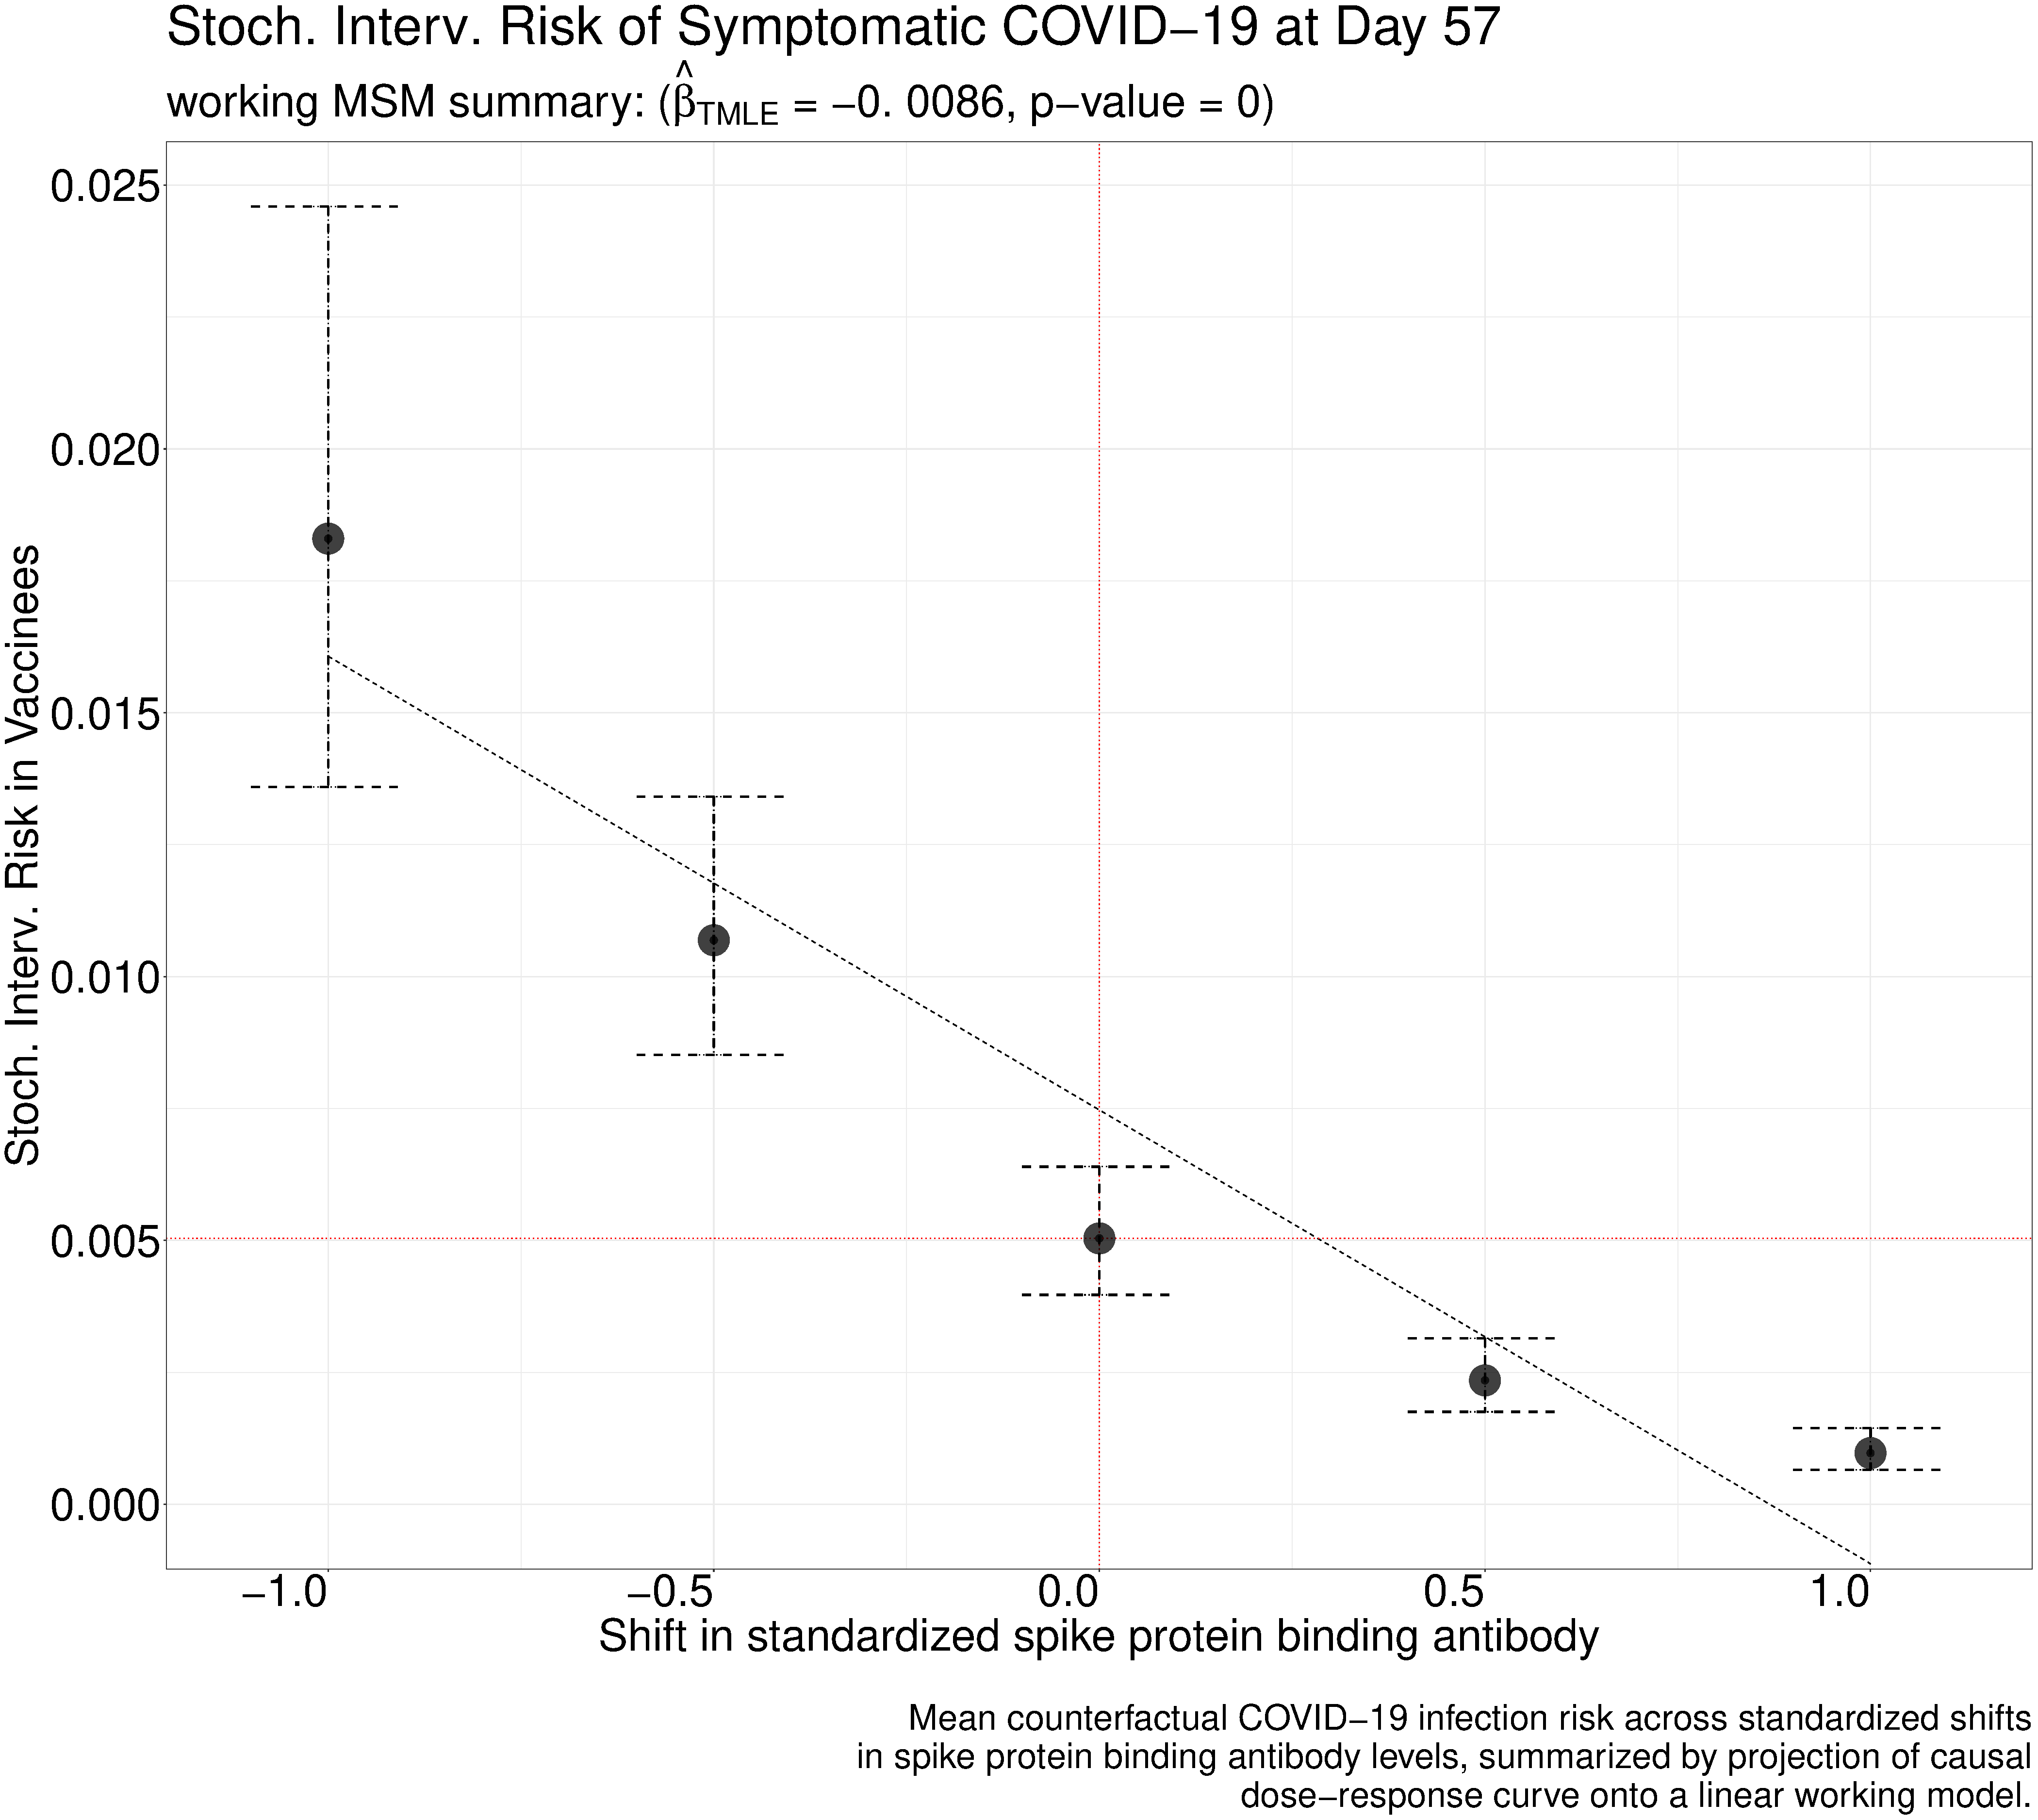
\includegraphics[width=0.975\linewidth,]{mcop_risk_Day57bindSpike}
  \caption{Stochastic interventional risk estimates, with confidence intervals,
  for the spike protein binding antibody at Day 57.}
  \label{fig:marker1-risk-day57}
\end{figure}

Estimation of the stochastic interventional risk for the spike protein antibody
across several values of $\delta$ reveals a monotonic decrease in risk with
increases in the activity of this immunologic marker. In particular, at $\delta
= 0$, for the vaccine administered in the current efficacy trial, the estimated
risk of symptomatic COVID-19 infection at Day 57 is 0.5\%. For positive values
of $\delta$, reflecting increased activity of the spike protein antibody, the
estimated risk of the adverse endpoint decreases towards zero. This suggests
that improvements to the dosage or formulation of the current vaccine may be
capable of improving its efficacy further still. Considering now negative values
of $\delta$, it appears that even moderate decreases in the modulation of this
antibody marker can significantly limit the efficacy of the vaccine against
infection. For example, with $\delta = -0.5$, the estimated risk doubles to
1.00\%; moreover, risk appears to grow sharply with further decreases in marker
activity. To summarize the trend in the change in estimated risk across the grid
in $\delta$, we note that projection onto a working marginal structural model
(MSM; as per Chapter~\ref{two}) yields a linear form with slope
$\hat{\beta}_{\text{TMLE}} = -0.0086$ and corresponding p-value of $p < 0.001$
for the hypothesis test of no trend (i.e., $H_0: \beta = 0$ and $H_1: \beta
\neq 0$).

\begin{figure}[H]
  \centering
  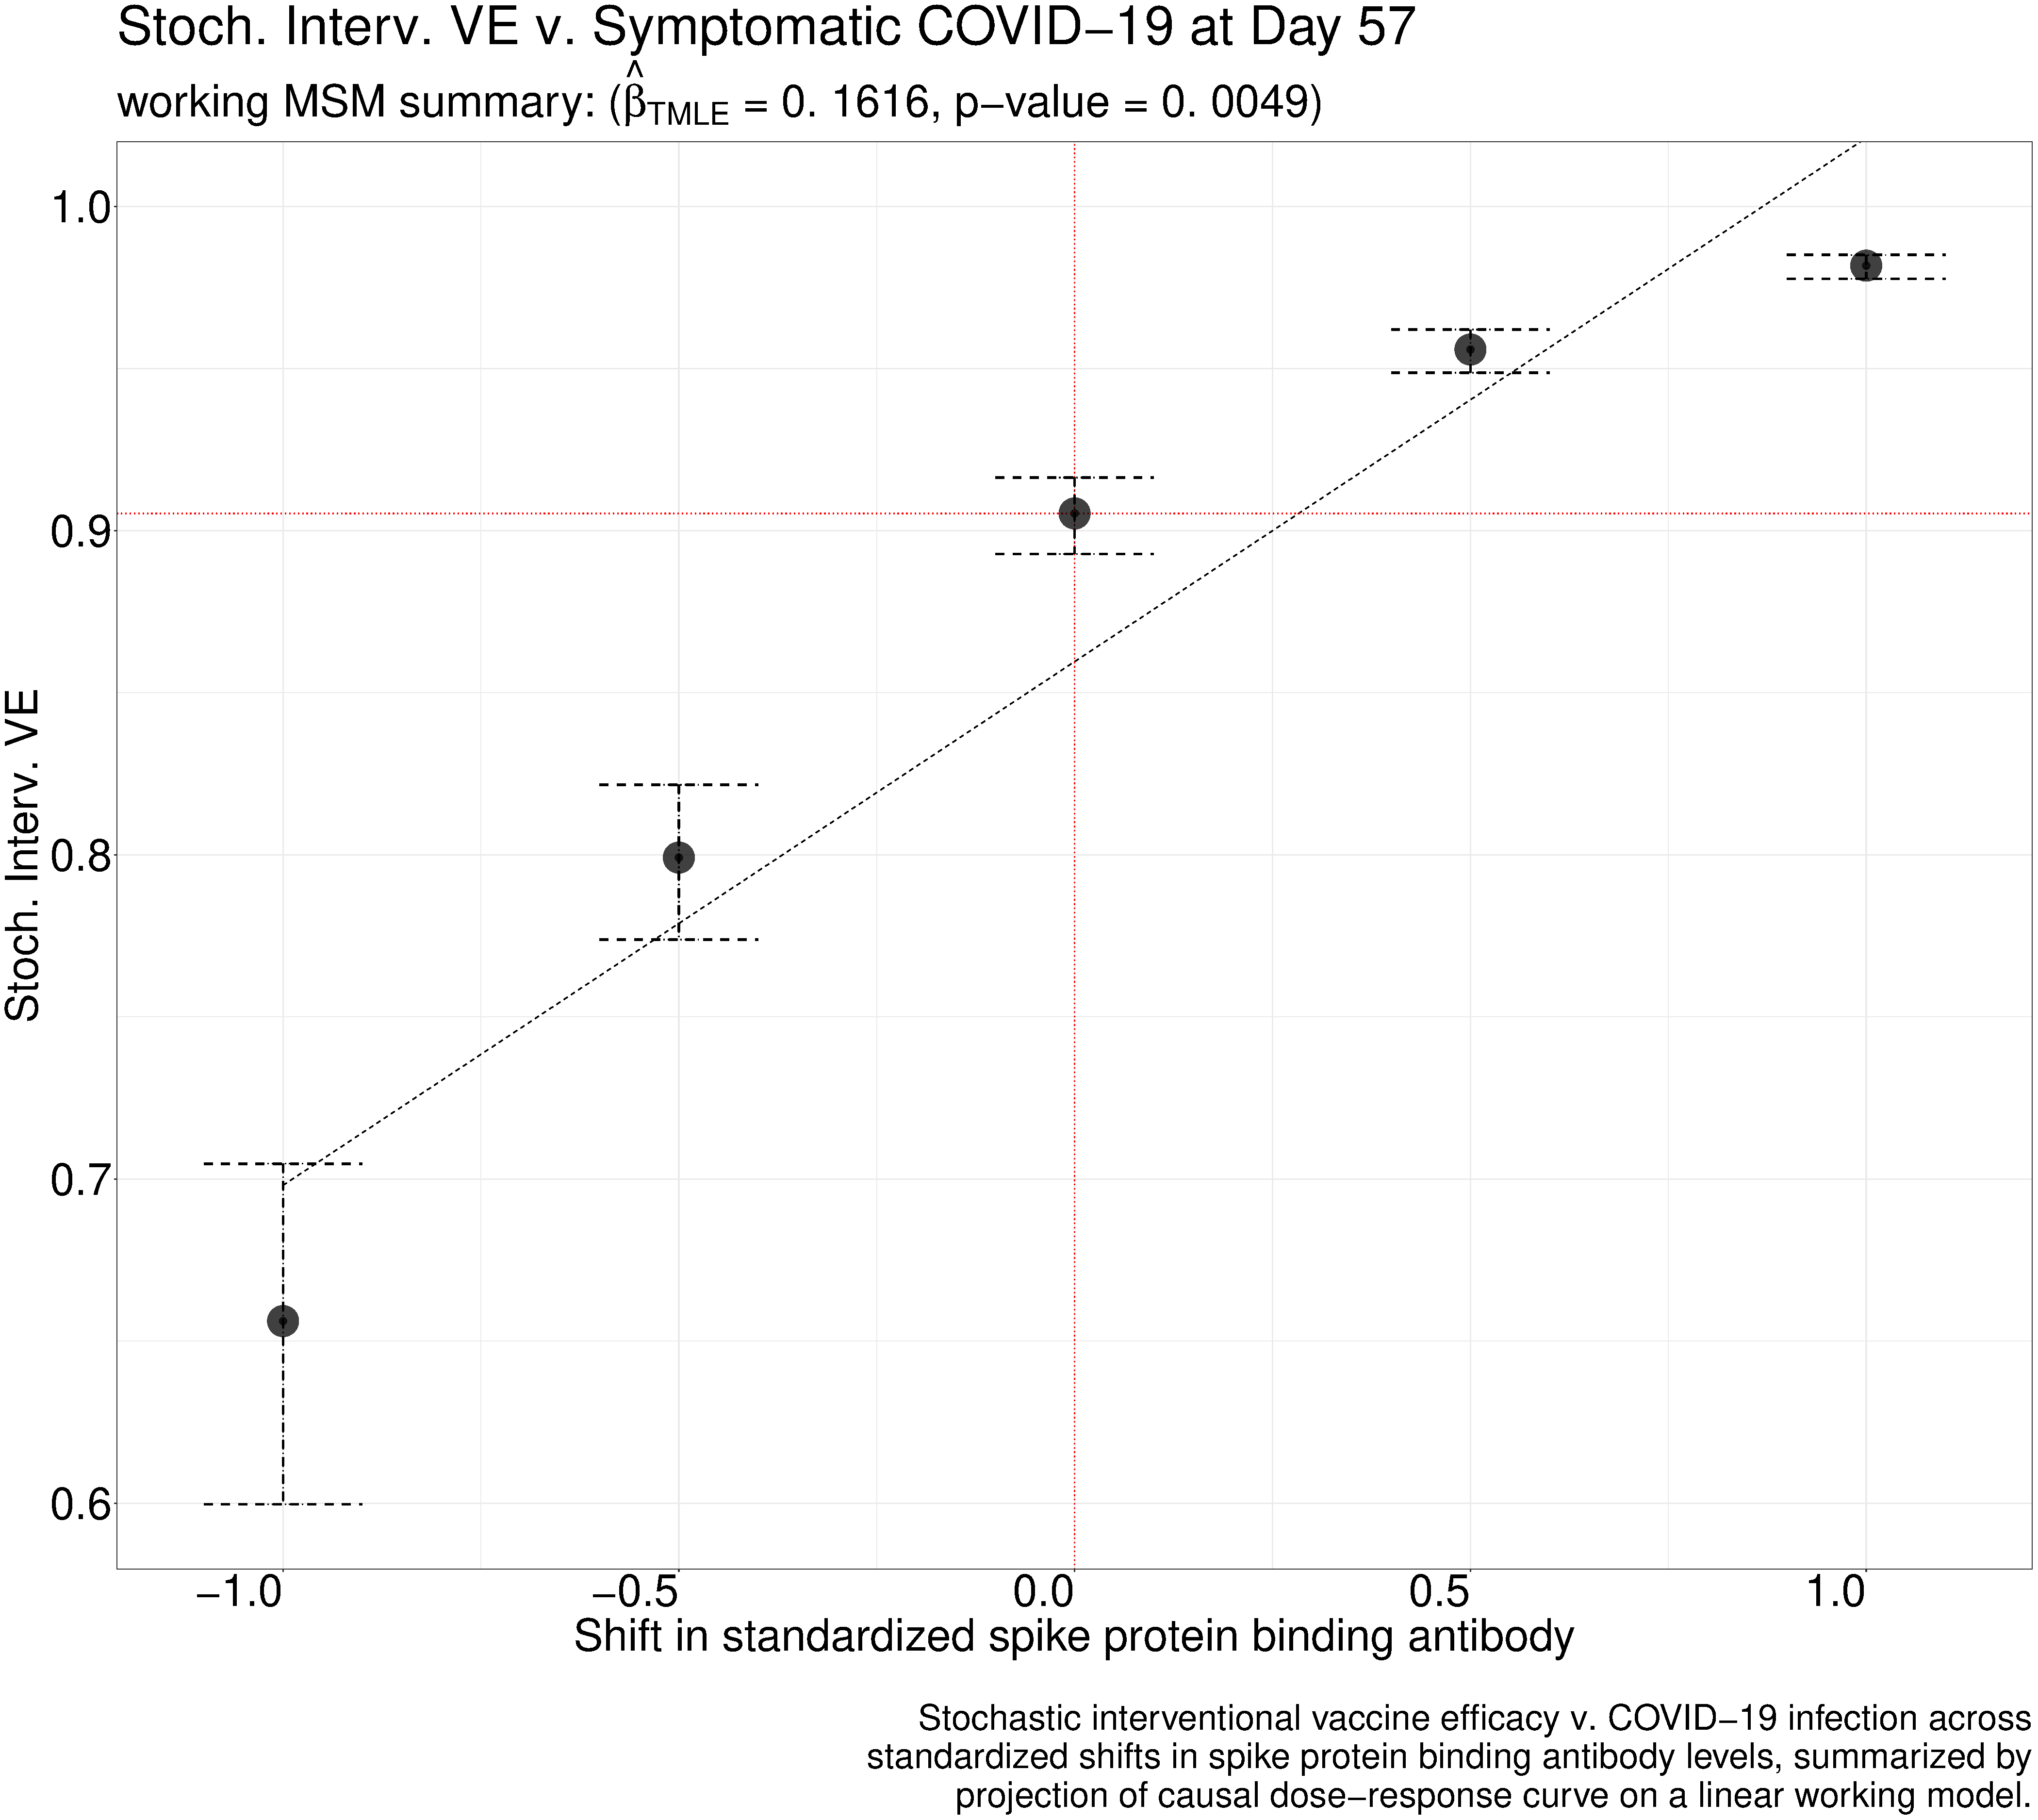
\includegraphics[width=0.975\linewidth,]{mcop_sve_Day57bindSpike}
  \caption{Stochastic interventional VE estimates, with confidence intervals,
    for the spike protein binding antibody at Day 57.}
  \label{fig:marker1-sve-day57}
\end{figure}

The evaluation of stochastic interventional VE is a process of re-scaling the
corresponding stochastic interventional risk estimates by the risk of infection
in the placebo arm of the trial, as per equation~\eqref{eqn:sve}. Accordingly,
the estimated VE provides information similar to that provided by the risk
estimates. In the case of the spike protein antibody, we find that the VE
produced by the administered vaccine (i.e., at $\delta = 0$) is just over 90\%.
What's more, upwards shifts of the activity of this marker have moderate impacts
on the estimated VE, with vaccine efficacy estimates of roughly 95\% and 97\%
for $\delta = 0.5$ and $\delta = 1$, respectively. While this analysis suggests
that reconstituting a future vaccine so as to specifically increase the activity
of the spike protein antibody may lead to very limited increases in protection,
the risk estimates at downwards shifts in its activity strongly suggest that all
vaccines ought to seek to module this marker at the level at which the current
vaccine does so. Specifically, a decrease of just a half standard unit (i.e.,
$\delta = -0.5$) leads to an estimated risk of 80\%, while a decrease of a full
standard unit ($\delta = -1$) yields a risk estimate of about 65\% --- 10\% and
25\% lower, respectively, than the risk estimate for the administered vaccine.
Examination of how VE estimates vary along the grid in $\delta$ reveals a sharp
increasing trend for the projection of the VE estimates onto a linear working
MSM. The slope parameter of the MSM is estimated to be
$\hat{\beta}_{\text{TMLE}} = 0.1616$ with a p-value of $p < 0.01$ for the
hypothesis test of no trend.

\begin{figure}[H]
  \centering
  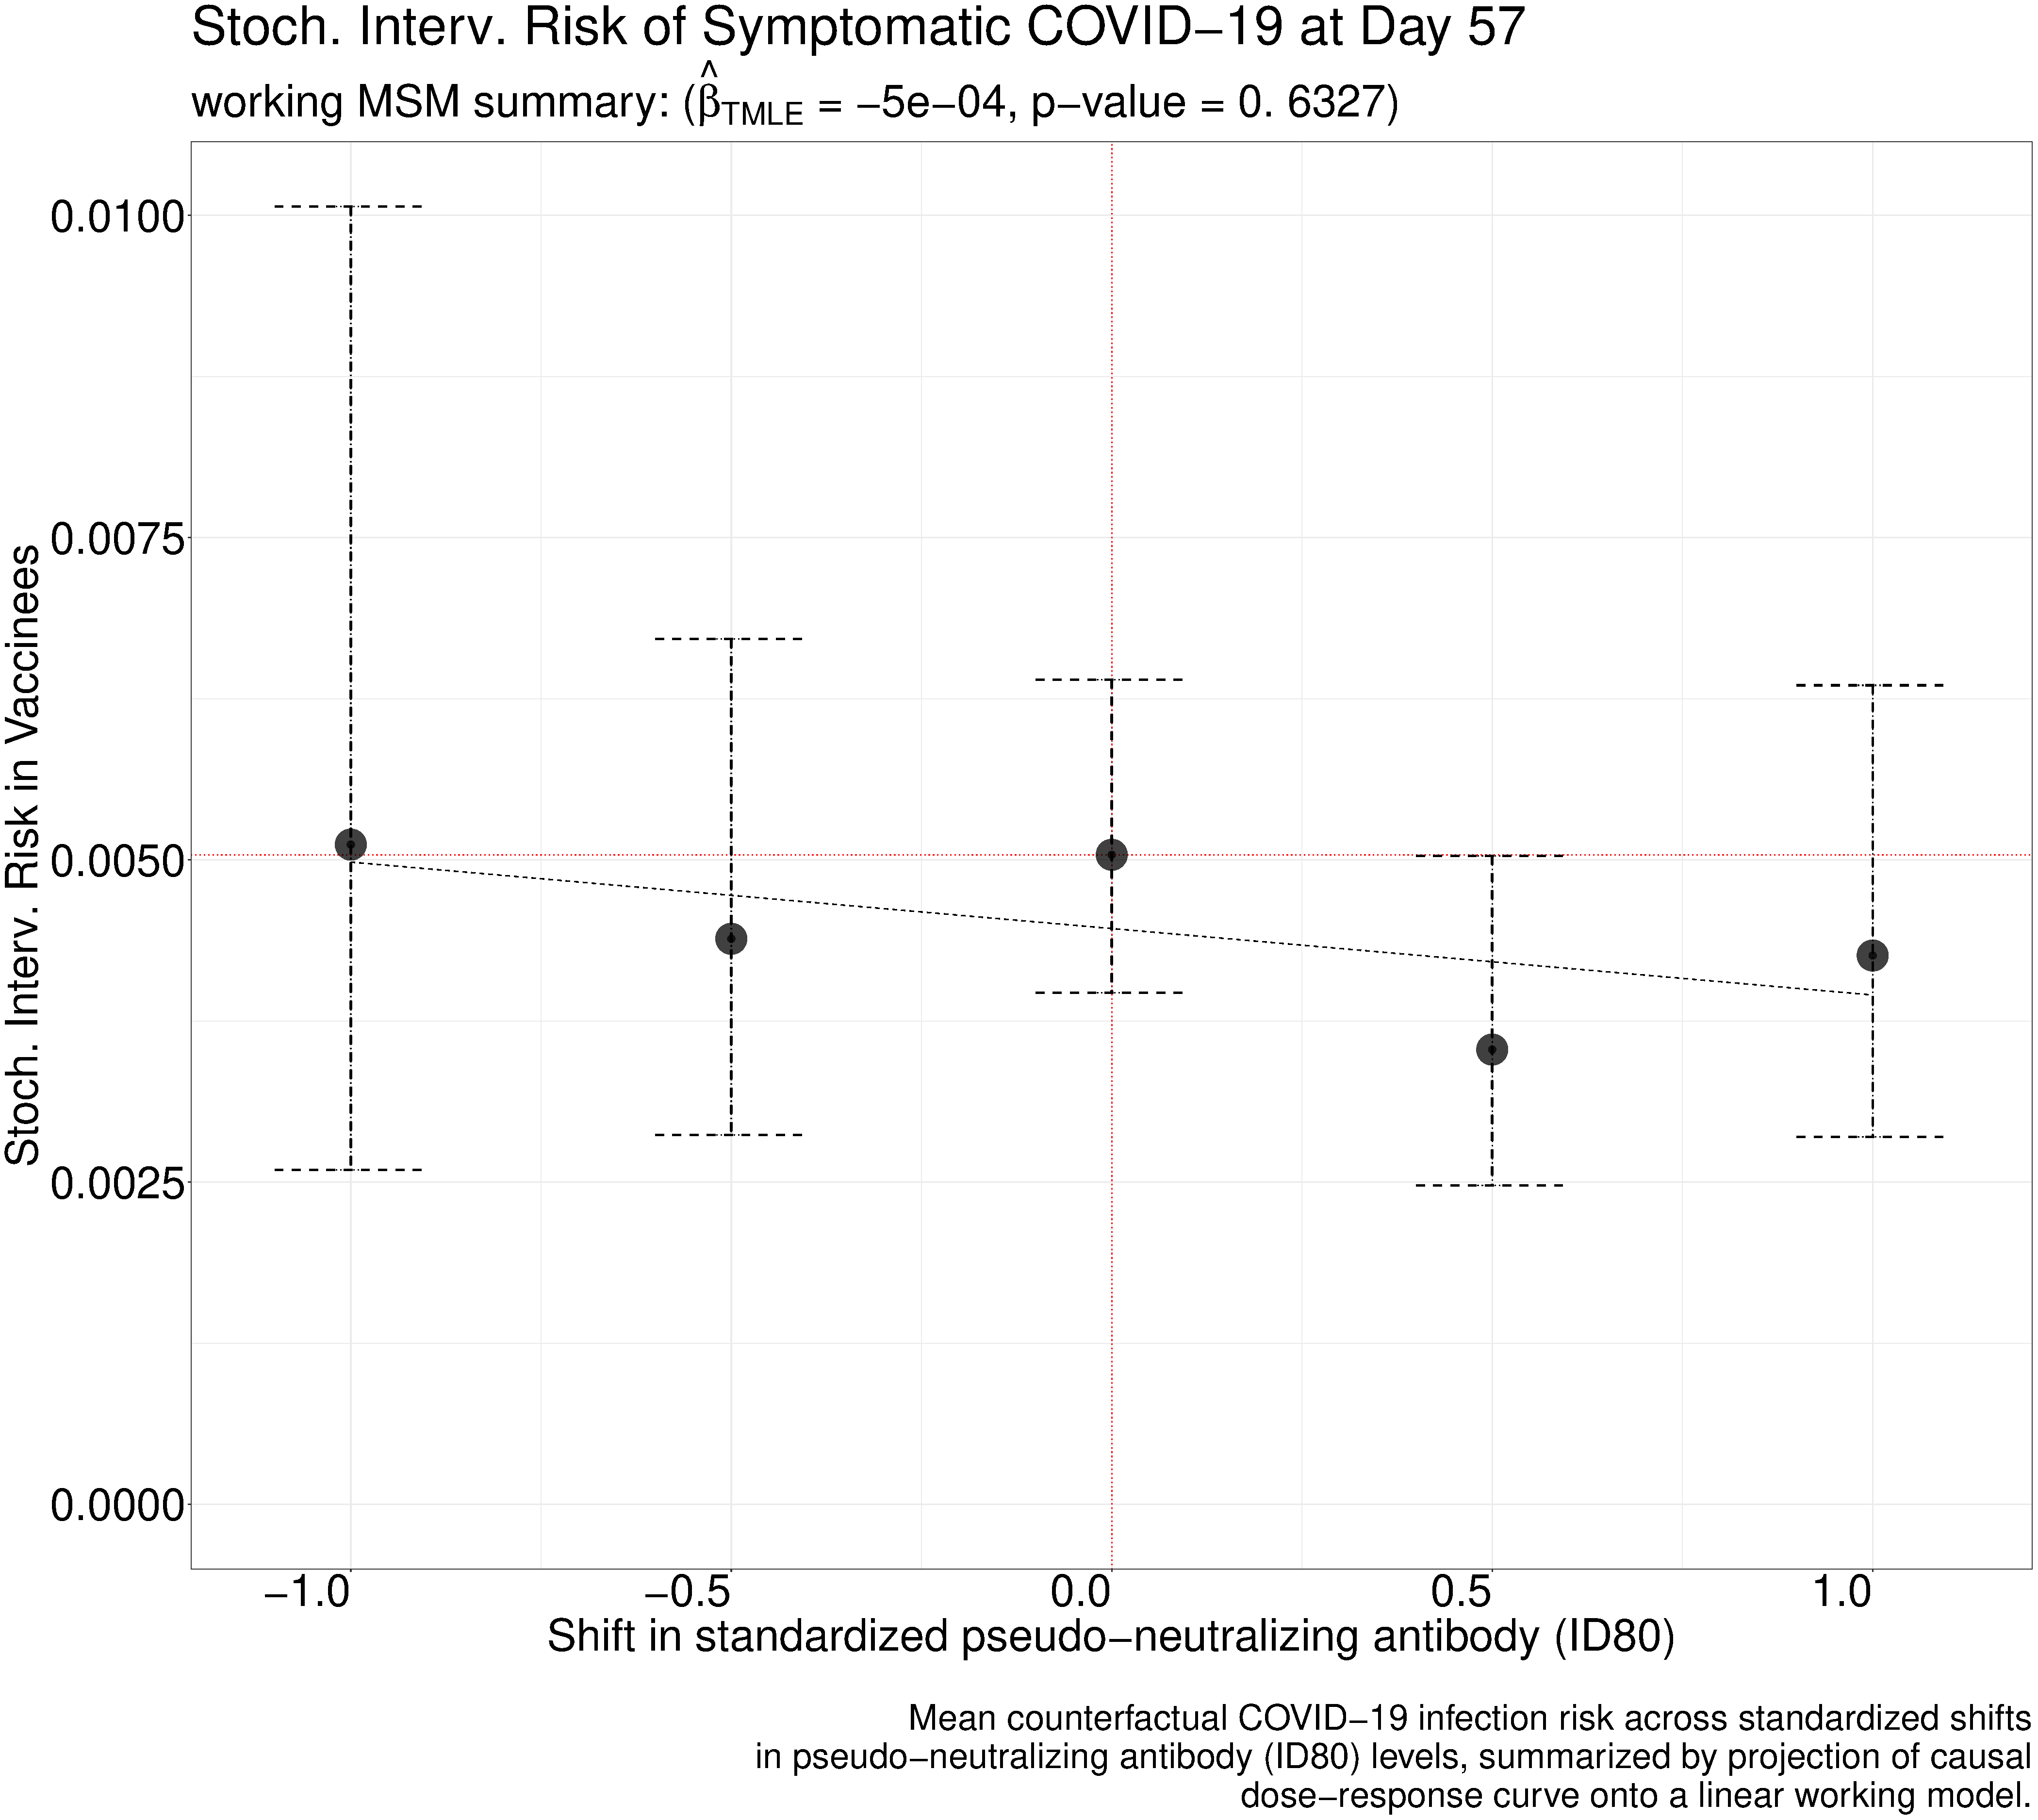
\includegraphics[width=0.975\linewidth,]{mcop_risk_Day57pseudoneutid80}
  \caption{Stochastic interventional risk estimates, with confidence intervals,
  for the pseudo-neutralizing antibody at Day 57.}
  \label{fig:marker4-risk-day57}
\end{figure}

Estimation of the stochastic interventional risk for the pseudo-neutralizing
antibody across the grid in $\delta$ reveals that the estimated risk is largely
insensitive to hypothetical changes in the marker activity. To start,
considering $\delta = 0$ (i.e., the activity of $S$ induced by the currently
administered vaccine), estimated risk of symptomatic COVID-19 infection at Day
57 is 0.5\%. The estimated stochastic interventional risk lies close to this
value for other values of $\delta$, suggesting that the pseudo-neutralizing
antibody may not be a suitable target for designing future vaccines to further
curb the risk of symptomatic COVID-19 infection.

\begin{figure}[H]
  \centering
  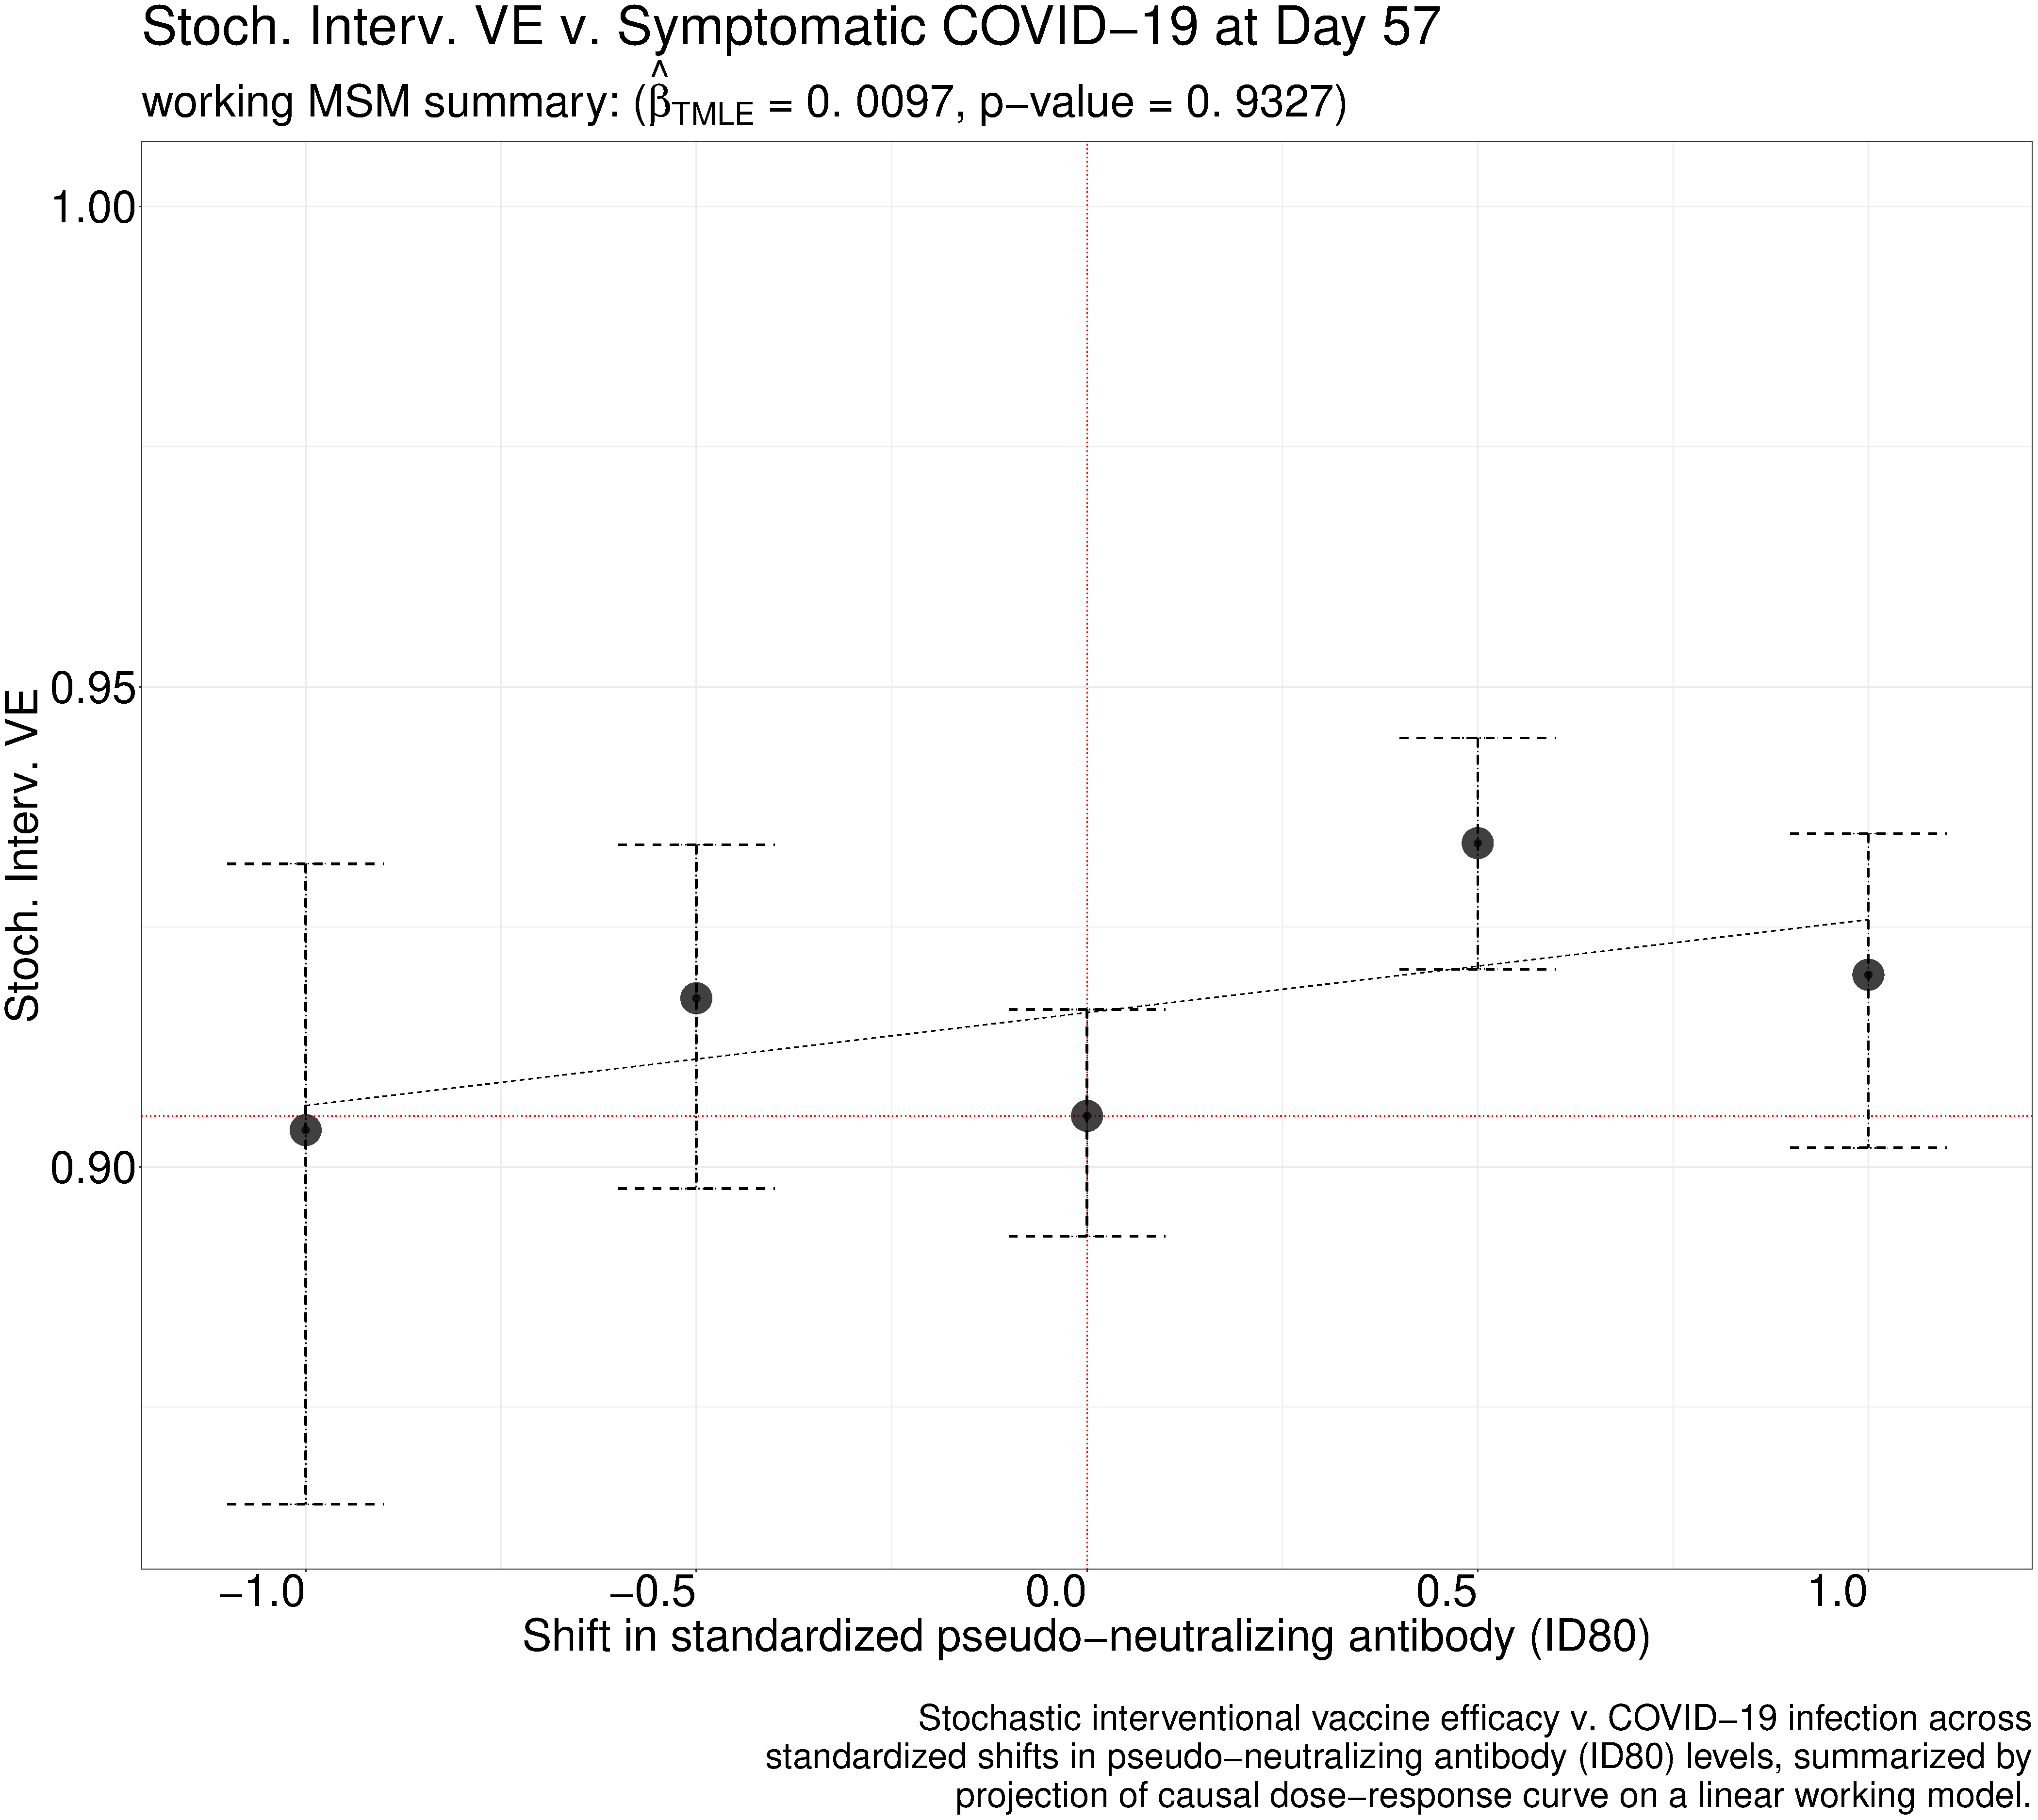
\includegraphics[width=0.975\linewidth,]{mcop_sve_Day57pseudoneutid80}
  \caption{Stochastic interventional VE estimates, with confidence intervals,
  for the pseudo-neutralizing antibody at Day 57.}
  \label{fig:marker4-sve-day57}
\end{figure}

Similarly to the estimates of the stochastic interventional risk for shifting of
the pseudo-neutralizing antibody, the stochastic VE estimates all lie within
roughly 3\% of the estimated VE at the null shift of $\delta = 0$. Examining the
VE estimate at that shift, we note an efficacy of roughly 90\%, with no sharp or
consistent changes in VE estimates at upwards or downwards shifts of the
activity of this marker. Consistent with the risk analyses, these VE estimates
suggest the pseudo-neutralizing antibody to be an unpromising candidate for
targeting by future vaccines.
